% Packages and settings:
%%%%%%%%%%%%%%%%%%%%%%%%%%%%%%%%%%%%%%%%%%
\documentclass[aspectratio=169]{beamer}
\usepackage[utf8]{inputenc}
\usepackage[english]{babel}
\usepackage{xeCJK}
\usepackage{hyperref}
\usepackage{tcolorbox}
\usepackage{tikz}
\usetikzlibrary{patterns}
\hypersetup{
    colorlinks=true,
    linkcolor=.,
    filecolor=magenta,      
    urlcolor=blue,
    citecolor=UGAblue,
}
\setbeamercovered{transparent}
\usepackage{appendixnumberbeamer}
\setbeamertemplate{caption}[numbered]{}

\usepackage{adjustbox} % Shrink stuff

%\usepackage[style=authoryear,sorting=ynt]{biblatex}
%\addbibresource{library.bib}
\usepackage[round]{natbib}
\bibliographystyle{unsrtnat}

\usetheme{Mateuszuga_wide}


% Title stuff:
%%%%%%%%%%%%%%%%%%%%%%%%%%%%%%%%%%%%%%%%%%
\title[Living Like There's No Tomorrow]{Living Like There's No Tomorrow:}
\subtitle{The psychological impacts of an earthquake on savings and spending behavior}
\author{Mateusz Filipski, Ling Jin, Xiaobo Zhang, Kevin Chen}
\institute{UGA, Huazhong Agricultural U., Beijing U., Zhejiang U., IFPRI}
\date{Virginia Tech, Oct 28, 2020}
\titlegraphic{
\includegraphics[width=3cm]{pics/UGAlogoWhiteTxt.png}}

\setcounter{showSlideNumbers}{1}

%%%%%%%%%%%%%%%%%%%%%%%%%%%%%%%%%%%%%%%%%%%%%%%%%%%%%%%%
% Begin document:
%%%%%%%%%%%%%%%%%%%%%%%%%%%%%%%%%%%%%%%%%%%%%%%%%%%%%%%%
\begin{document}

\frame{\titlepage}

%%%%%%%%%%%%%%%%%%%%%%%%%%%%%%%%%%%%%%%%%%%%%%%%%%%%%%%%
%% Introduction
%%%%%%%%%%%%%%%%%%%%%%%%%%%%%%%%%%%%%%%%%%%%%%%%%%%%%%%%
\section*{Introduction}
\begin{frame}[label=top]
    \frametitle{\Large{LaFontaine was not so great at biology}}
    \begin{columns}
    \begin{column}{0.5\textwidth}
        \begin{itemize}
            \item French Playwright and satirist (1622-1673) (莫里哀)
            \item Famous for his "Fables" (stories about animals with morals for humans)
            \item Most famous: 
            The Cicada and The Ant
        \end{itemize}
    \end{column}
    \begin{column}{0.5\textwidth}  %%<--- here
    \begin{center}
    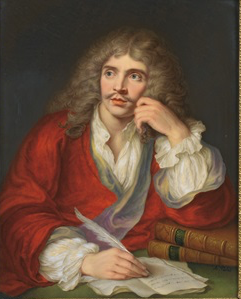
\includegraphics[scale=0.55]{pics/moliere.png}     \end{center}
\end{column}
\end{columns}
\end{frame}  

\begin{frame}[label=top]
    \frametitle{\Large{Moral: Cicada should have saved up for winter}}
    \begin{columns}
    \begin{column}{0.4\textwidth}
        \begin{itemize}
            \item Cicada sings all summer, while Ant works and saves 
            \item Come winter: Cicada begs Ant for food
            \newline
            \item Nice story, but there's a problem.
        \end{itemize}
    \end{column}
    \begin{column}{0.6\textwidth}  %%<--- here
    \begin{center}
    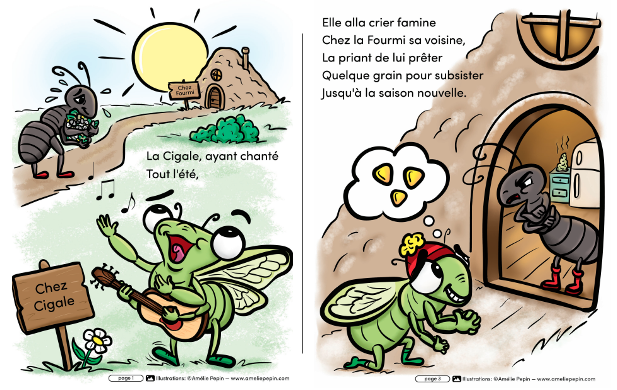
\includegraphics[scale=0.40]{pics/cigaleFourmi2.png}
    {\tiny source: \href{https://www.ameliepepin.com/}{ameliepepin.com}}
    \end{center}
    \end{column}
    \end{columns}
\end{frame}  

\begin{frame}[label=top]
    \frametitle{\Large{Question: What do Cicadas do in the winter?}}
    \begin{columns}
        \begin{column}{0.5\textwidth}
            \begin{itemize}
                \item \textbf{Answer}: They die! 
                \item Ants live several years: survive winters in their ant-hills
                \item Adult cicadas live \textit{only in summer}: they come out of the ground, reproduce, lay eggs, and die.  
                \newline
                \pause
                \item Cicada has \textbf{no incentive whatsoever} to store food
            \end{itemize}
        \end{column}
        \begin{column}{0.5\textwidth}  %%<--- here
        \begin{center}
            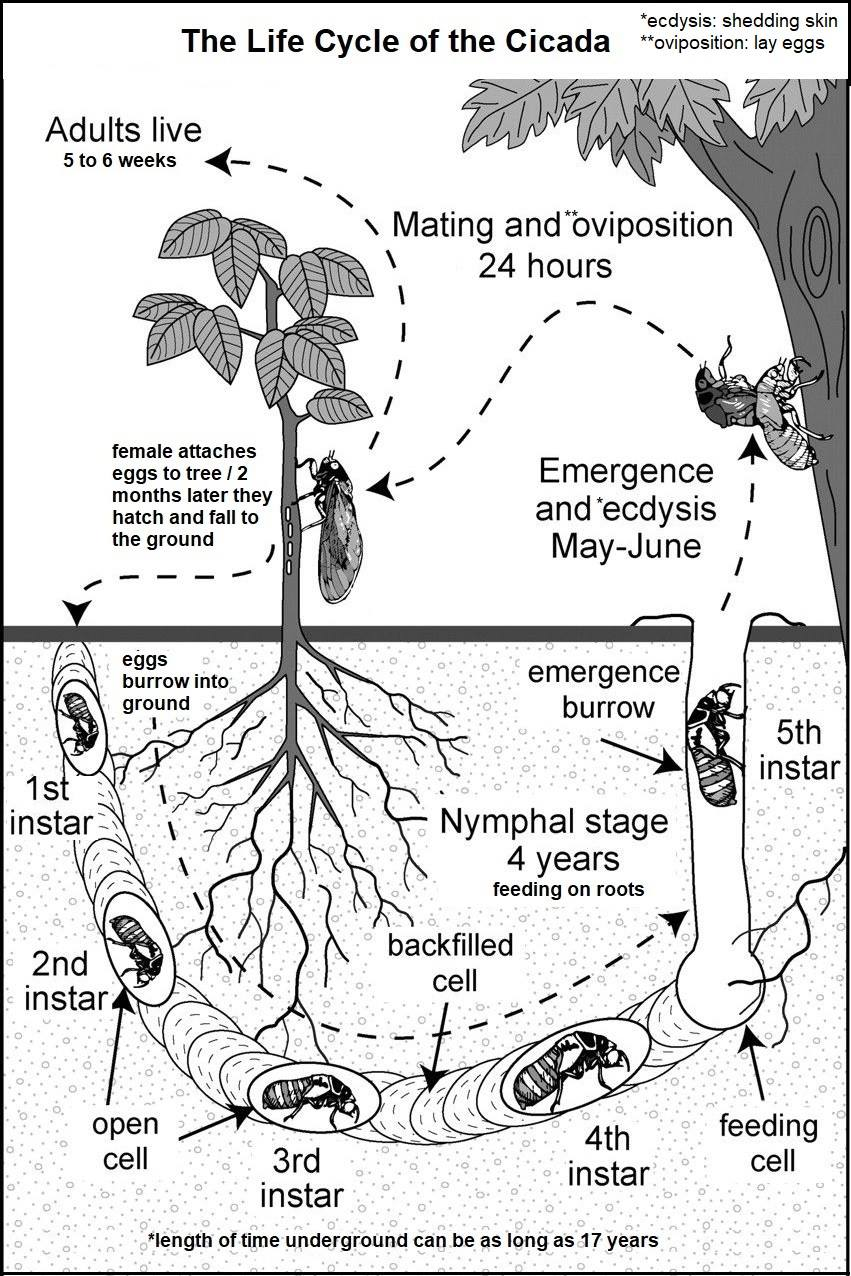
\includegraphics[scale=0.16]{pics/cicada_life_cycle.jpg}.   
            {\tiny source: \href{https://thehouseholdpests.org/cicada-life-cycle-images.html}{thehouseholdpests.com}}
        \end{center}
    \end{column}
    \end{columns}
\end{frame}  

% \begin{frame}[label=top]
%     \frametitle{\Large{A similar insight underpins the paper}}
%     \begin{itemize}
% 		\item How do people change their behavior after a disaster?  
% 		\item Might save more, take fewer risks (to survive the next disaster) 
% 		\item ... but might save less, and take more risks (because they might die anyways)
% 	\end{itemize}  
% 	\vspace{0.5cm}
% 	\pause
%     \begin{tcolorbox}{}
%     \textit{Life is so unpredictable. People can leave us anytime.}\\ --- Villager in Wenchuan, 2008
%     \end{tcolorbox} 
%     \vspace{0.5cm}
% 	\pause
% 	This paper uses the Sichuan earthquake to see which effect dominates. 
% \end{frame}  

\begin{frame}[label=top]
    \frametitle{\Large{A similar insight underpins the paper}}
    \begin{itemize}
		\item How do people change their behavior after a disaster?  
		\item Especially: Saving + Risk-taking
		\item We use the 2008 Sichuan earthquake to shed some light. 
	\end{itemize}
\end{frame}  


\begin{frame}
    \frametitle{\LARGE{Motivation from the field}}
    \begin{itemize}
		\item What changed after the Sichuan earthquake? 
		\item Our expectation: people protect themselves against the next earthquake
		\begin{itemize}
		    \item Saving more
		    \item Working to generate buffer incomes
		    \item Become more "Ant-like"
		\end{itemize}
		\item <2-> Informal interviews: 
		    People play Majiang more. "Enjoy life while it lasts"
		\begin{itemize}
		    \item More "Cicada-like"
		\end{itemize}
		\item <3-> Could this at odds with economic theory? 
		
	\end{itemize}  
\end{frame}  

\begin{frame}
    \frametitle{\LARGE{How do people act when facing risk?}}
	\begin{itemize}
		\item Theory mostly says: People facing risk act conservatively (as long as they are risk-averse).
		\item Lots of literature supports this: 
		\begin{itemize}
		    \item Consumption smoothing, savings, income smoothing, diversification...
		    \item Micro-level: \cite{Udry1995}  Nigerian rural households save in anticipation of weather shocks
		    \item Behavioral econ: \cite{Cameron2013} Increased and persistent risk aversion if suffered a disaster in Indonesia. 
		    \item Macro-level: \cite{Skidmore2001} cross-country reg. Disasters correlated with higher savings (but this is rather weak)
		\end{itemize}
	\end{itemize}
\end{frame} 

\begin{frame}
    \frametitle{\LARGE{But sometimes the opposite seems true}}
	\begin{itemize}
		\item ``Nothing to lose" theory \citep{Harris2002} 
		\item Micro-level: Lower investment in education \citep{Fortson2011}, unsafe sexual behavior \citep{Oster2012}, drug use \citep{Gibbons2004}
		\item Behavioral econ: Risk-loving among Katrina evacuees \citep{Eckel2009} 
		\item Risk-loving, drinking and gambling after Great Japan Earthquake \citep{Hanaoka2018}  
	\end{itemize}
\end{frame} 


\begin{frame}
    \frametitle{\LARGE{Conundrum and central question:}}
	\begin{itemize}
		\item Literature suggests both reckless behavior and conservative behavior in the face of risk 
		\item Is it ``plan for the rainy day" or ``live like there's no tomorrow" 
	\end{itemize}
\end{frame} 

\begin{frame}
    \frametitle{\LARGE{How the paper contributes:}}
	\begin{itemize}
		\item Theoretical: Cast the conundrum within an economic framework
	    \begin{itemize}
		    \item Type of risk is what matters
		    \item Risk of loss vs. risk of death
		\end{itemize}
		\item Methodological: 
		    \begin{itemize} 
		        \item How can we test which dominates?
		        \item How to narrow down only the psychological effects?
		    \end{itemize}
		\item Empirical: Which tendency dominated after the Sichuan earthquake of 2008?
		\begin{itemize}
		    \item Saving money (primary focus)
		    \item Drinking alcohol
		    \item Playing Majiang
		\end{itemize}
	\end{itemize}
\end{frame} 

\begin{frame}
	\frametitle{\Large{Preview: Earthquake => Lower savings}}
	\begin{figure}
	    \caption{\small{Change in savings rate and distance to epicenter (\textcolor{red}{Unaffected households})}}
	    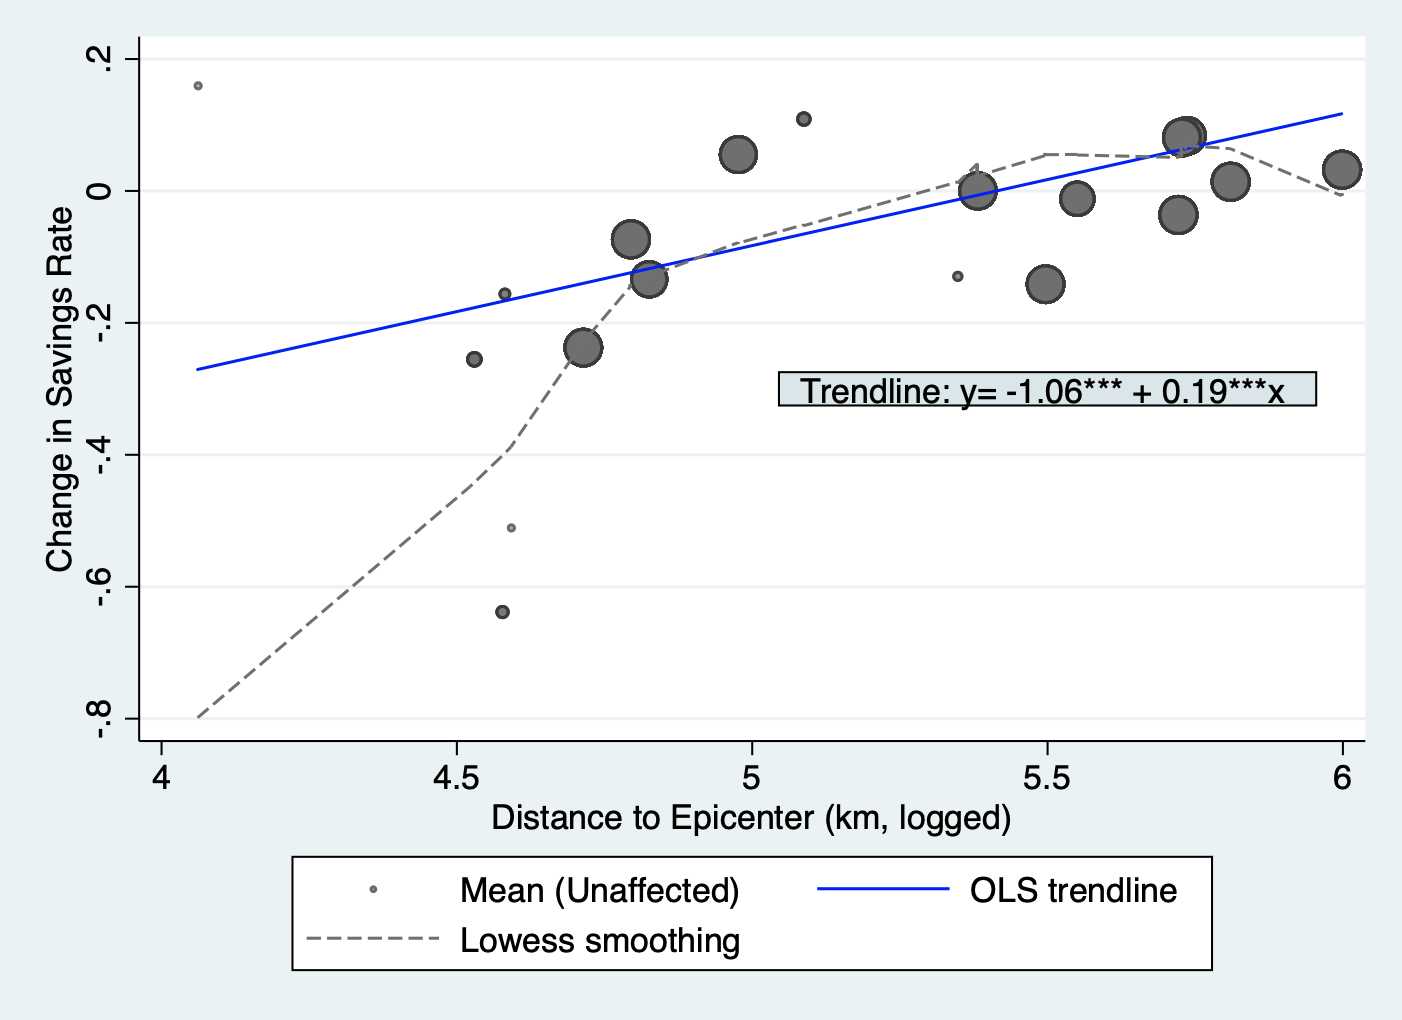
\includegraphics[scale=0.35]{pics/incomecons_plot_RAR2draft} 
	\end{figure}
\end{frame}


%%%%%%%%%%%%%%%%%%%%%%%%%%%%%%%%%%%%%%%%%%%%%%%%%%%%%%%%
%% Theory
%%%%%%%%%%%%%%%%%%%%%%%%%%%%%%%%%%%%%%%%%%%%%%%%%%%%%%%%
\section{Theory}
\begin{frame}
    \frametitle{\Large{Risk of loss is not the same as risk of death}}
    \begin{itemize}
        \item If I believe I might lose my wealth \\
            => Protect myself. Save to prevent future hardship. \\ 
            => ``Save for the rainy day"
        \item If I believe I might die before I can use my wealth \\ 
            => Spend everything now (no need to save for nothing) \\ 
            => ``Live like there's no tomorrow"
    \end{itemize}
\end{frame} 
	
\begin{frame}
    \frametitle{\Large{Tradeoff: consume now or later?}}
    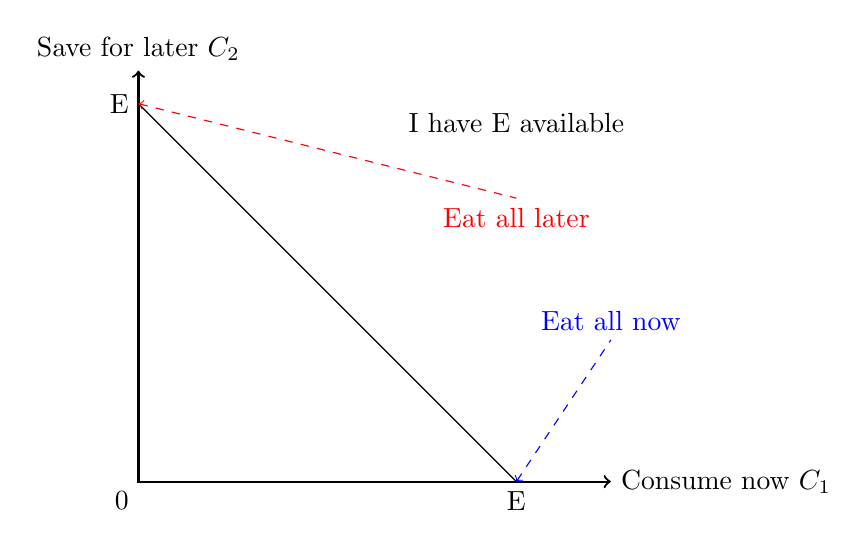
\begin{tikzpicture}[scale=0.6]
        \draw[thick,<->] (0,8.7) node[above]{Save for later $C_2$}--(0,0)--(10,0) node[right]{Consume now $C_1$};
        \node [below left] at (0,0) {$0$};
        \draw<2->(0,8)--(8,0) node[below]{E};
        \node<2-> [left] at (0,8) {E};
        \node<2-> [below] at (8,8) {I have E available};
        \draw<3-> [dashed, <-, red] (0,8)--(8,6) node[below]{Eat all later};
        \draw<3-> [dashed, <-, blue] (8,0)--(10,3) node[above]{Eat all now};
    \end{tikzpicture} \\
    I have no time preference, no income between the periods
\end{frame} 
	
\begin{frame}
    \frametitle{\Large{With no risk, I should split half-half}}
    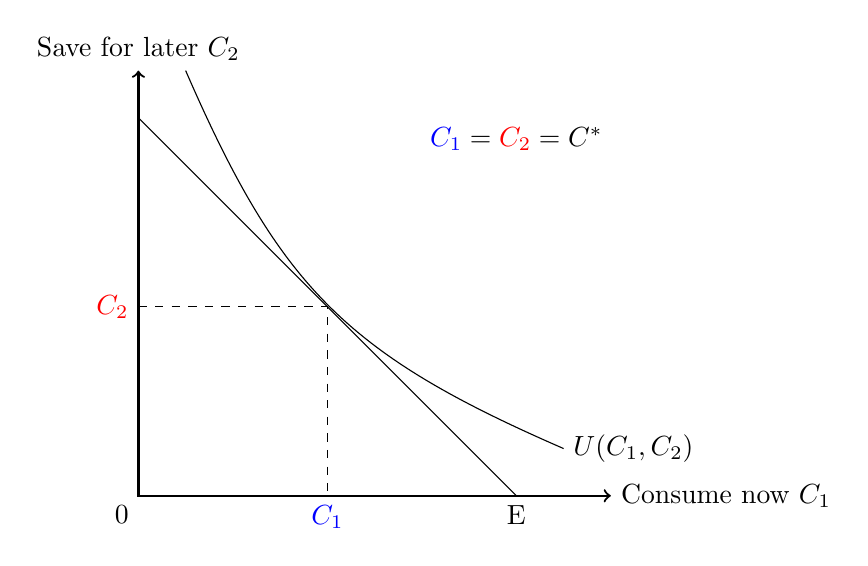
\begin{tikzpicture}[scale=0.6]
        \draw[thick,<->] (0,9) node[above]{Save for later $C_2$}--(0,0)--(10,0) node[right]{Consume now $C_1$};
        \node [below left] at (0,0) {$0$};
        \draw(0,8)--(8,0) node[below]{E};
        \node<2-> [below, blue] at (4,0) {$C_1$};
        \node<2-> [left, red] at (0,4) {$C_2$};
        \draw<2-> [dashed](0,4)--(4,4)--(4,0);
        \draw<2-> (1,9) ..controls (3,4.4) and (4.4,3) .. (9,1) node[right]{$U(C_1,C_2)$};
        \node<3-> [below] at (8,8) {$\textcolor{blue}{C_{1}}=\textcolor{red}{C_{2}}=C^*$};
    \end{tikzpicture}
\end{frame} 

\begin{frame}
    \frametitle{\Large{With risk of loss, I should keep more for later}}
    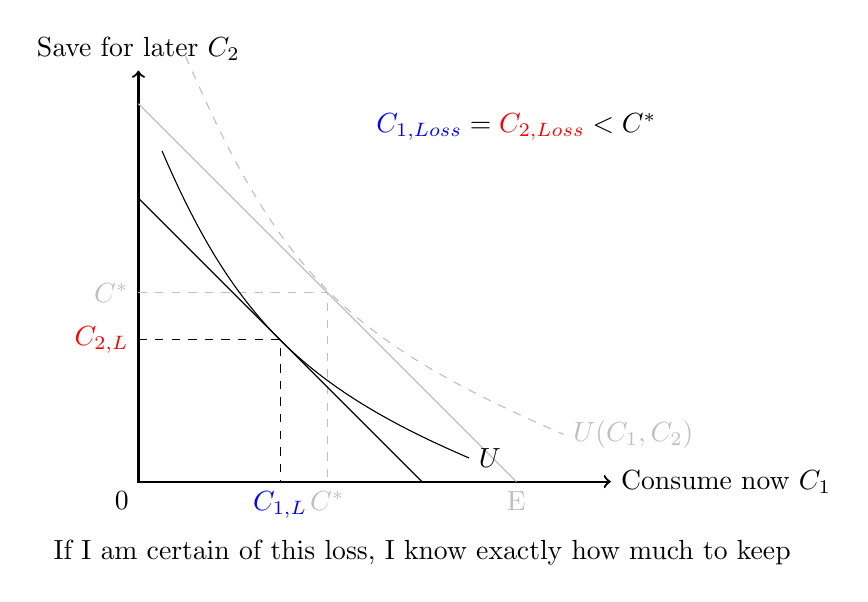
\begin{tikzpicture}[scale=0.6]
        \draw[thick,<->] (0,8.7) node[above]{Save for later $C_2$}--(0,0)--(10,0) node[right]{Consume now $C_1$};
        \node [below left] at (0,0) {$0$};
        \draw [gray!50] (0,8)--(8,0) node[below]{E};
        \node [below, gray!50] at (4,0) {$C^*$};
        \node [left, gray!50] at (0,4) {$C^*$};
        \draw [dashed, gray!50](0,4)--(4,4)--(4,0);
        \draw [dashed, gray!50] (1,9) ..controls (3,4.4) and (4.4,3) .. (9,1) node[right]{$U(C_1,C_2)$};
        \draw<2-> (0,6)--(6,0);
        \draw<2-> (0.5,7) ..controls (2,3.5) and (3.5,2) .. (7,0.5) node[right]{$U$};
        \draw<3-> [dashed] (0,3)--(3,3)--(3,0);
        \node<3-> [below, blue] at (3,0) {$C_{1,L}$};
        \node<3-> [left, red] at (0,3) {$C_{2,L}$};
        \node<3-> [below] at (8,8) {$\textcolor{blue}{C_{1,Loss}}=\textcolor{red}{C_{2,Loss}} < C^*$};
        \node<4-> [right] at (-2,-1.5) {If I am certain of this loss, I know exactly how much to keep};
    \end{tikzpicture} 
\end{frame} 

\begin{frame}
    \frametitle{\Large{With risk of death, I should eat more now}}
    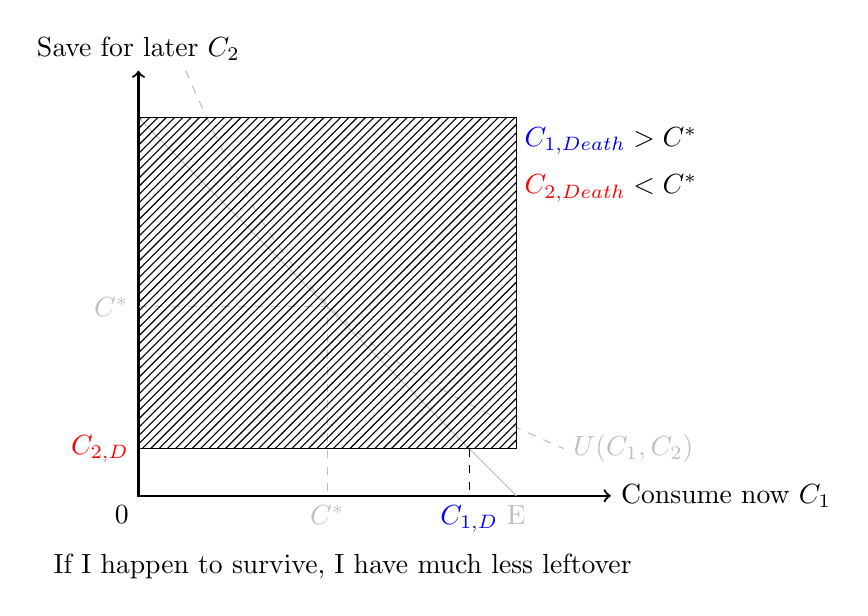
\begin{tikzpicture}[scale=0.6]
        \draw[thick,<->] (0,9) node[above]{Save for later $C_2$}--(0,0)--(10,0) node[right]{Consume now $C_1$};
        \node [below left] at (0,0) {$0$};
        \draw [gray!50] (0,8)--(8,0) node[below]{E};
        \node [below, gray!50] at (4,0) {$C^*$};
        \node [left, gray!50] at (0,4) {$C^*$};
        \draw [dashed, gray!50](0,4)--(4,4)--(4,0);
        \draw [dashed, gray!50] (1,9) ..controls (3,4.4) and (4.4,3) .. (9,1) node[right]{$U(C_1,C_2)$};
        \draw<2-> [pattern= north east lines] (0,1) rectangle (8,8);
        \draw<3-> [dashed] (7,1)--(7,0) ;
        \node<3-> [below] at (10,8){$\textcolor{blue}{C_{1,Death}}> C^*$};
        \node<3-> [below,blue] at (7,0) {$C_{1,D}$};
        \node<3-> [below] at (10,7){$\textcolor{red}{C_{2,Death}}< C^*$};
        \node<3-> [left,red] at (0,1) {$C_{2,D}$};
        \node<4-> [right] at (-2,-1.5) {If I happen to survive, I have much less leftover};
    \end{tikzpicture} 
\end{frame} 

\begin{frame}
    \frametitle{\Large{Let's explore this using data}}
    \begin{itemize}
        \item Do people save more or save less after a disaster?
        \item Can we isolate the psychological impact? 
        \item <2-> Bonus: Do we see the conflict between loss vs. death? 
    \end{itemize}
\end{frame} 



%%%%%%%%%%%%%%%%%%%%%%%%%%%%%%%%%%%%%%%%%%%%%%%%%%%%%%%%
%% Methodology
%%%%%%%%%%%%%%%%%%%%%%%%%%%%%%%%%%%%%%%%%%%%%%%%%%%%%%%%
\section{Methodology}
\begin{frame}
    \frametitle{\Large{Goal: Show this finding is robust}}
	\begin{figure}
	    \caption{\small{Change in savings rate and distance to epicenter (Unaffected households)}}
	    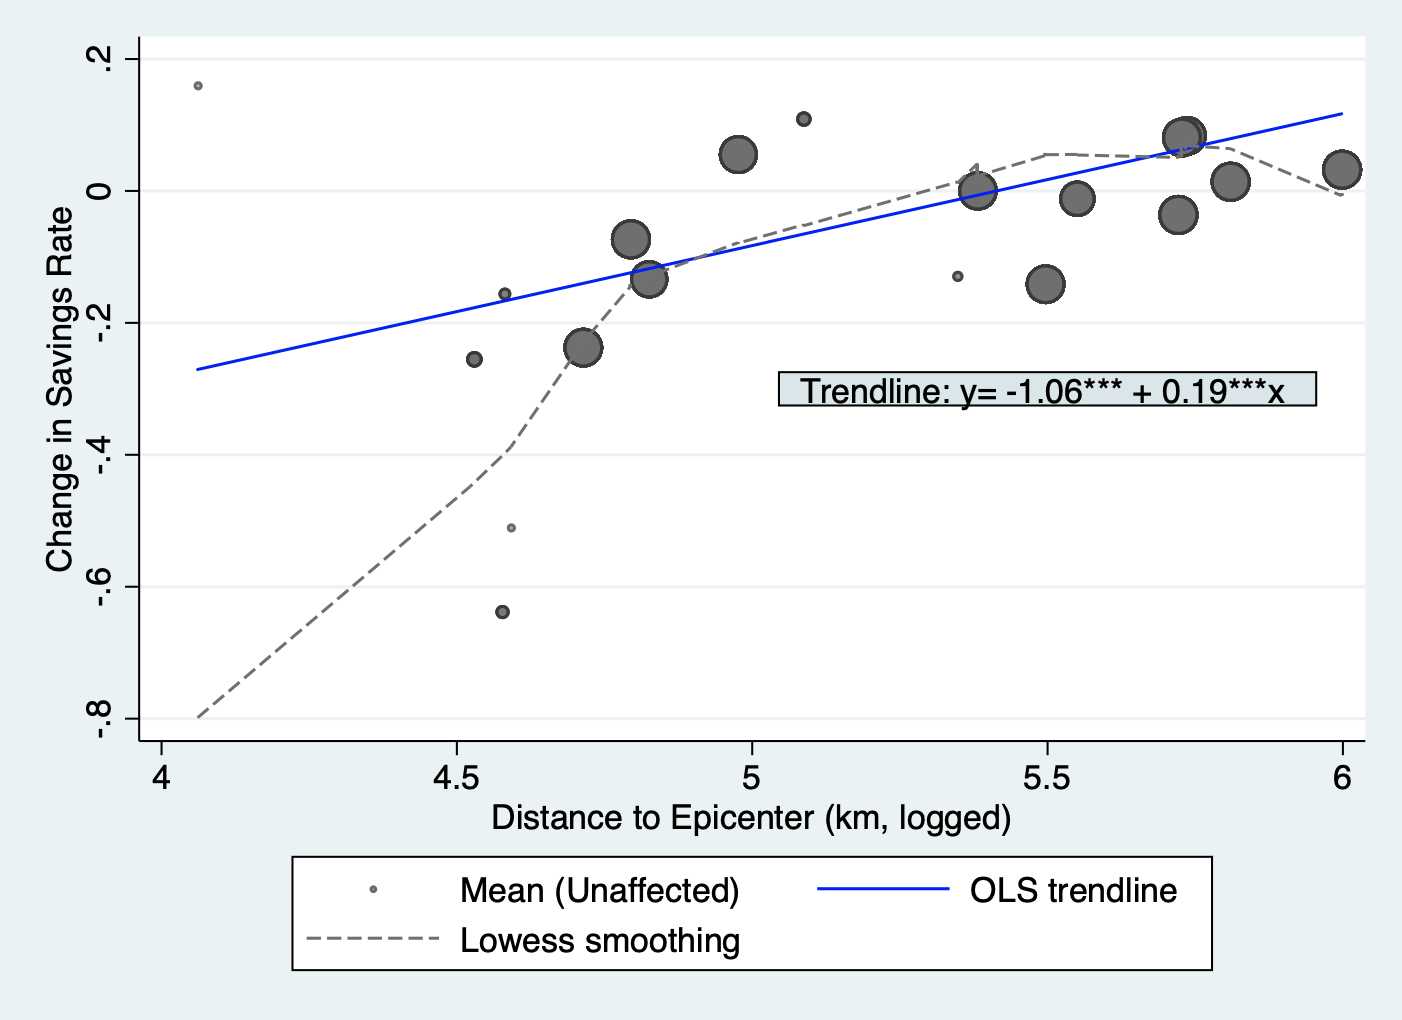
\includegraphics[scale=0.35]{pics/incomecons_plot_RAR2draft} 
	\end{figure}
\end{frame}
\begin{frame}[label=simpleQuestion]
    \frametitle{\LARGE{A simple question?}}
    Obvious idea = first-difference regression before/after the disaster:
    \begin{equation}
        \Delta s_h = \beta + \gamma I_h + \delta X_h + \eta \Delta Z_h + \epsilon
    \end{equation}
	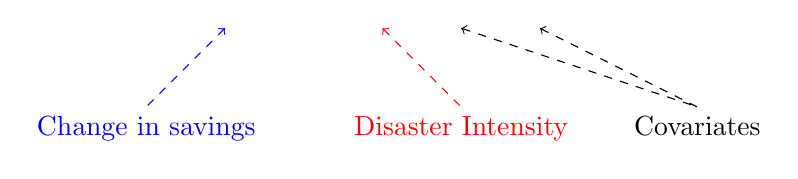
\begin{tikzpicture}   %% use here too
        \draw [dashed, <-, blue] (7,3)--(6,2) node[below]{Change in savings};
        \draw [dashed, <-, red] (9,3)--(10,2) node[below]{Disaster Intensity};
        \draw [dashed, <-, black] (10,3)--(13,2) node[below]{Covariates};
        \draw [dashed, <-, black] (11,3)--(13,2) ;
    \end{tikzpicture} \\
    \begin{itemize}
        \item<2-> There are challenges with that: \\
        \begin{itemize}
            \item How to measure intensity? Damages are endogenous \hyperlink{threeLittlePigs}{\beamergotobutton{why?}}
            \item Reconstruction expenditures influence savings
            \item<3-> The first issue is a ``bias" issue, the second is a ``story" issue
        \end{itemize}
    \end{itemize}
\end{frame}


\begin{frame}
\frametitle{\LARGE{Solving the issues}}
\begin{itemize}
	\item Solving the ``bias" issue:
	\begin{itemize}
		\item Need an \textbf{exogenous} ($\approx$random) measure of intensity 
		\item Earthquake is good for that: epicenter is random. 
		\item We use distance to epicenter 
	\end{itemize}
	\item<2-> Solving the ``story" issue:
	\begin{itemize}
		\item Need to isolate the \textbf{psychological} impacts
		\item We restrict to households who were not economically affected  
		\item Home not damaged, no injuries, no deaths, etc...  
\end{itemize}

\end{itemize}
\end{frame}


\begin{frame}
	\frametitle{\LARGE{Regression specification}}
	The idea is essentially to regress this:
	\begin{equation}
	\Delta s_{h| \textcolor{blue}{unaffected}} = \beta + \gamma \textcolor{red}{D_v} + \delta X_h + \eta \Delta Z_h +  \epsilon
	\end{equation}
	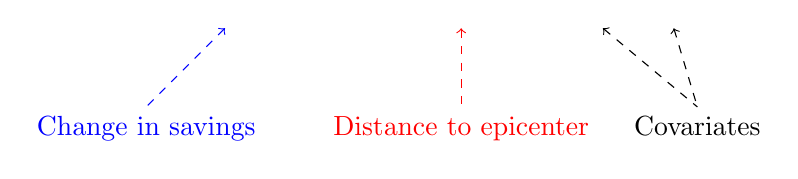
\begin{tikzpicture}   %% use here too
	\draw [dashed, <-, blue] (2,3)--(1,2) node[below]{Change in savings};
	\draw [dashed, <-, red] (5,3)--(5,2) node[below]{Distance to epicenter};
	\draw [dashed, <-, black] (6.8,3)--(8,2) node[below]{Covariates};
	\draw [dashed, <-, black] (7.7,3)--(8,2) ;
	\end{tikzpicture} 
\end{frame}


\begin{frame}
	\frametitle{\LARGE{Regression specification}}
	In prectice we use a continuous diff-in-diff specification:
	\begin{equation}
		s_{h,t| \textcolor{blue}{unaffected}} = \beta 
		+ \zeta \textcolor{teal}{T_t} 
		+ \mathbf{\xi} \textcolor{red}{T_t*D_v}
		+ \eta Z_{h,t} 
		+ \lambda H_h
		+ \epsilon	
	\end{equation}
	\begin{tikzpicture}[overlay]   %% use here too
		\draw [dashed, <-, teal] (6,3)--(4,2.5) node[below]{Post-earthquake};
		\draw [dashed, <-, red] (7.3,3)--(6.3,2) node[below]{Distance x Post-earthquake };
		\draw [dashed, <-, black] (10.3,3)--(12,1) node[below]{Household fixed-effects};
	\end{tikzpicture} \\
	\begin{itemize}
		\item<2-> The coefficient of interest is $\xi$ 
		\begin{itemize}
			\item If positive, it means further distance => higher savings
			\item (i.e. closer distance => lower savings) 
			\item Because of our sample, we can say it is psychological
		\end{itemize}
	\end{itemize}
\end{frame}


%%%%%%%%%%%%%%%%%%%%%%%%%%%%%%%%%%%%%%%%%%%%%%%%%%%%%%%%
%% Data
%%%%%%%%%%%%%%%%%%%%%%%%%%%%%%%%%%%%%%%%%%%%%%%%%%%%%%%%
\section{Data}
\begin{frame}
	\frametitle{The Sichuan Earthquake was deadly}
	\begin{itemize}
		\item Earthquake on May 12th, 2008, Magnitude 8
		\begin{itemize}
			\item Killed tens of thousands
			\item Injured hundreds of thousands
			\item Left five million homeless 
			\item Tremendous emotional shock 
		\end{itemize}
		\item <2-> Huge investment in reconstruction 
		\begin{itemize}
			\item Officially over by 2011 
		\end{itemize}
	\end{itemize}
\end{frame}


\begin{frame}
	\frametitle{Map of our survey locations}
	\vspace{0.5cm}
	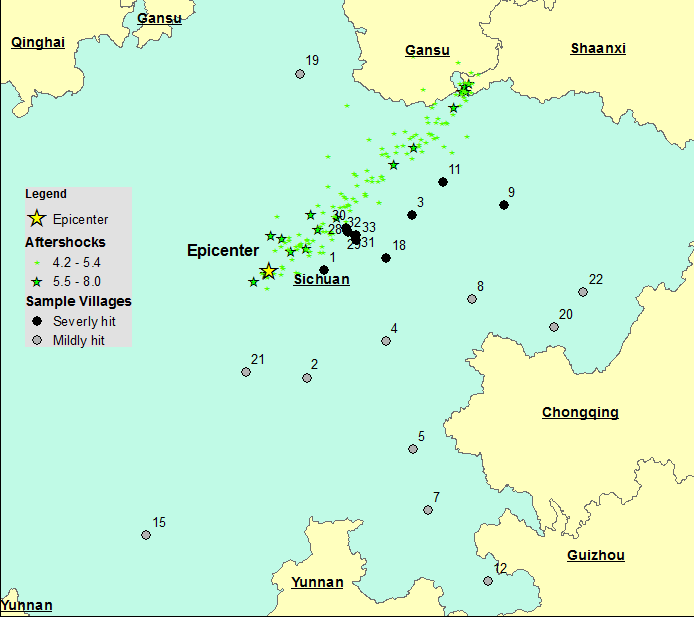
\includegraphics[scale=0.45]{pics/MapSichuanQuakeForPaper_v2_latest_cropped} \\	
\end{frame}


\begin{frame}
\frametitle{We built a 3-year panel dataset}
	\begin{itemize}
		\item Two rural household surveys merged
		\begin{itemize}
			\item The Sichuan Rural Household and Migration Survey (SRHMS)
			\item The Sichuan component of RCRE
		\end{itemize}
		\item <2-> SRHMS 
		\begin{itemize}
			\item 6 villages of 2 townships in Mianzhu County, Sichuan
			\item Three waves: 2007, 2009, and 2011
			\item Around 800 sample households
		\end{itemize}
		\item <3-> RCRE
		\begin{itemize}
			\item Annual national rural household survey, since 1984 (we use 07, 09, 11)
			\item In Sichuan: 16 villages, about 800 households
			\item Around 800 sample households
		\end{itemize}
	\end{itemize}
\end{frame}


\begin{frame}
	\frametitle{Important variables}
	\vspace{0.6}
	\begin{table}
		\centering
		\caption{\label{tab:sumstats} \small{Some of the variables used in the analysis} }
		\small
		{
\def\sym#1{\ifmmode^{#1}\else\(^{#1}\)\fi}
\begin{tabular}{l*{1}{cc}}
\hline\hline
                    &\multicolumn{2}{c}{(1)}  \\
                    &\multicolumn{2}{c}{Stats}\\
                    &        mean&          sd\\
\hline
\textbf{Explained variables:}&            &            \\
Savings Rate [ln(Y/C)]&       0.626&       0.671\\
Frequency playing majiang (times/month)&       3.171&       7.001\\
Expenditures on alcohol (RMB)&      63.008&      87.412\\
\textbf{Control variables:}&            &            \\
Income per capita (ln)&       9.885&       0.855\\
Job loss in household&       0.118&       0.322\\
CPI (village)       &      91.281&       7.625\\
Gifts given (RMB 1k)&       0.018&       0.123\\
Loans given (RMB 1k)&       0.038&       0.240\\
Gvt. aid (RMB 1k)   &       0.445&       0.651\\
\hline
Observations        &        1767&            \\
\hline\hline
\end{tabular}
}

	\end{table}
\end{frame}	

%%%%%%%%%%%%%%%%%%%%%%%%%%%%%%%%%%%%%%%%%%%%%%%%%%%%%%%%
%% Results
%%%%%%%%%%%%%%%%%%%%%%%%%%%%%%%%%%%%%%%%%%%%%%%%%%%%%%%%
\section*{Results}
\begin{frame}
	\frametitle{\Large{Core result: Earthquake => Lower savings}}
	\begin{figure}
	    \caption{\small{Change in savings rate and distance to epicenter (Unaffected households)}}
	    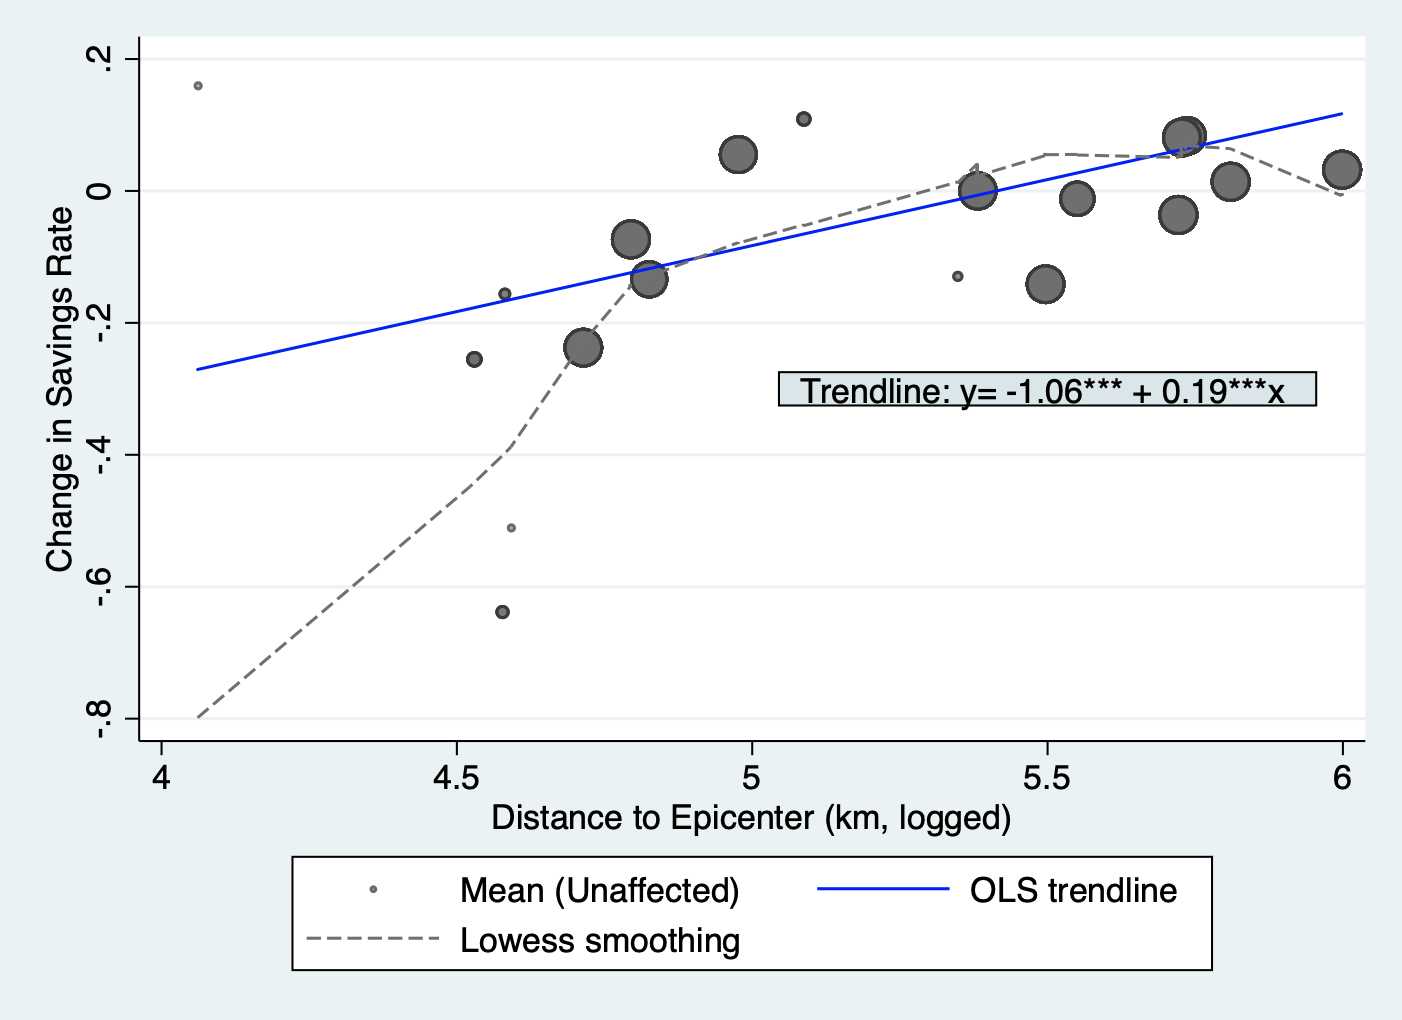
\includegraphics[scale=0.35]{pics/incomecons_plot_RAR2draft} 
	\end{figure}
\end{frame}

%	\includegraphics[scale=0.4]{pics/regressions} 

\begin{frame}
	\frametitle{Core result holds when regressing}
	\begin{table}[p]
		\centering
		\caption{\label{tab:reg1} \small{Impact of earthquake on savings rate, unaffected households}}
		\small
		{
\def\sym#1{\ifmmode^{#1}\else\(^{#1}\)\fi}
\begin{tabular}{l*{1}{c}}
\hline\hline
                    &\multicolumn{1}{c}{(1)}\\
                    &\multicolumn{1}{c}{Sav. Rate}\\
\hline
\textbf{Explanatory Variables:}&                    \\
[1em]
Ln(Distance) x 2009 &       0.156\sym{**}\\
                    &      (2.46)        \\
[1em]
Ln(Distance) x 2011 &       0.167        \\
                    &      (1.64)        \\
[1em]
Household controls included &         Yes        \\
\hline
Observations        &        1767        \\
Households          &         589        \\
Adjusted R-sq.      &       0.015        \\
\hline\hline
\multicolumn{2}{l}{\footnotesize HH controls: gender, age, party member, education, hh size, land}\\
\end{tabular}
}

	\end{table}
\end{frame}

\begin{frame}
\frametitle{\Large{Possible explanations for this coefficient}}
\begin{itemize}
	\item "Income Hypothesis" 
	\item "Inflation Hypothesis" 	
	\item "Altruism Hypothesis" 
	\item "Non-fungibility Hypothesis" 
	\item "No Tomorrow Hypothesis" 
\end{itemize}
\end{frame}


\begin{frame}
\frametitle{Ruling out other explanations}
    \begin{table}[p]
    	\centering
    	\fontsize{8pt}{8pt}\selectfont
    	{
\def\sym#1{\ifmmode^{#1}\else\(^{#1}\)\fi}
\begin{tabular}{l*{5}{c}}
\hline\hline
                    &\multicolumn{1}{c}{(1)}&\multicolumn{1}{c}{(2)}&\multicolumn{1}{c}{(3)}&\multicolumn{1}{c}{(4)}&\multicolumn{1}{c}{(5)}\\
                    &\multicolumn{1}{c}{Sav. Rate}&\multicolumn{1}{c}{Sav. Rate}&\multicolumn{1}{c}{Sav. Rate}&\multicolumn{1}{c}{Sav. Rate}&\multicolumn{1}{c}{Sav. Rate}\\
\hline
\textbf{Explanatory Variables:}&                    &                    &                    &                    &                    \\
Ln(Distance) x 2009 &       0.156\sym{**}&       0.172\sym{**}&       0.173\sym{**}&       0.174\sym{**}&       \textbf{0.170\sym{**}}\\
                    &      (2.46)        &      (2.42)        &      (2.33)        &      (2.32)        &      (2.36)        \\
Ln(Distance) x 2011 &       0.167        &       0.227\sym{**}&       0.230\sym{**}&       0.229\sym{**}&       \textbf{0.228\sym{**}}\\
                    &      (1.64)        &      (2.72)        &      (2.78)        &      (2.72)        &      (2.72)        \\
Income per capita (ln)&                    &       0.795\sym{**}&       0.795\sym{**}&       0.794\sym{**}&       0.795\sym{**}\\
                    &                    &     (26.89)        &     (26.90)        &     (26.78)        &     (26.84)        \\
Job loss in household&                    &     -0.0542        &     -0.0543        &     -0.0559        &     -0.0547        \\
                    &                    &     (-1.48)        &     (-1.48)        &     (-1.53)        &     (-1.50)        \\
CPI (village)       &                    &                    &     0.00106        &     0.00124        &     0.00128        \\
                    &                    &                    &      (0.23)        &      (0.26)        &      (0.27)        \\
Gifts given (RMB 1k)&                    &                    &                    &      0.0437        &      0.0464        \\
                    &                    &                    &                    &      (0.42)        &      (0.44)        \\
Loans given (RMB 1k)&                    &                    &                    &     -0.0255        &     -0.0262        \\
                    &                    &                    &                    &     (-0.73)        &     (-0.75)        \\
Gvt. aid (RMB 1k)   &                    &                    &                    &                    &    -0.00951        \\
                    &                    &                    &                    &                    &     (-0.39)        \\
Household controls  &         Yes        &         Yes        &         Yes        &         Yes        &         Yes        \\
\hline
Observations        &        1767        &        1767        &        1767        &        1767        &        1767        \\
Households          &         589        &         589        &         589        &         589        &         589        \\
Adjusted R-sq.      &       0.015        &       0.547        &       0.546        &       0.546        &       0.546        \\
\hline\hline
\multicolumn{6}{l}{\footnotesize \tiny{Includes all previous controls}}\\
\end{tabular}
}

    \end{table}
    \begin{tikzpicture}   
    	\draw<2-> [overlay, color = red]  (10,5.9) rectangle (11.5,7.2);
    \end{tikzpicture}
\end{frame}

\begin{frame}
    \frametitle{\Large{Earthquake increased alcohol expenditures}}
    \begin{table}
    	\centering
    	\scriptsize		{
\def\sym#1{\ifmmode^{#1}\else\(^{#1}\)\fi}
\begin{tabular}{l*{2}{c}}
\hline\hline
                    &\multicolumn{1}{c}{(1)}&\multicolumn{1}{c}{(2)}\\
                    &\multicolumn{1}{c}{OLS, FE}&\multicolumn{1}{c}{Tobit, RE}\\
\hline
Effects on alcohol expenditures:&                    &                    \\
Ln(Distance) x 2009 &      \textbf{-19.95\sym{*}} &      \textbf{-24.97\sym{**}}\\
                    &     (-1.75)        &     (-2.36)        \\
Ln(Distance) x 2011 &      \textbf{-23.93\sym{**}}&      \textbf{-31.29\sym{**}}\\
                    &     (-2.20)        &     (-2.96)        \\
Household controls  &         Yes        &         Yes        \\
Hypotheses controls &         Yes        &         Yes        \\
\hline
Observations        &        1767        &        1767        \\
Households          &         589        &         589        \\
Adjusted R-sq.      &       0.031        &                    \\
Chi-sq.             &                    &     157.614        \\
\hline\hline
\multicolumn{3}{l}{\footnotesize \tiny{Includes all previous controls}}\\
\end{tabular}
}

    \end{table}
\end{frame}

\begin{frame}
\frametitle{\Large{Earthquake increased Majiang frequency}}
\begin{table}
	\centering
	\scriptsize		{
\def\sym#1{\ifmmode^{#1}\else\(^{#1}\)\fi}
\begin{tabular}{l*{3}{c}}
\hline\hline
                    &\multicolumn{1}{c}{(1)}&\multicolumn{1}{c}{(2)}&\multicolumn{1}{c}{(3)}\\
                    &\multicolumn{1}{c}{OLS, FE}&\multicolumn{1}{c}{Poisson, FE}&\multicolumn{1}{c}{Tobit, RE}\\
\hline
Effects on frequency playing majiang:&                    &                    &                    \\
Ln(Distance) x 2011 &      \textbf{-0.850\sym{**}}&      \textbf{-0.407\sym{**}}&      \textbf{-3.301\sym{**}}\\
                    &     (-2.34)        &     (-2.64)        &     (-2.65)        \\
Household controls  &         Yes        &         Yes        &         Yes        \\
Hypotheses controls &         Yes        &         Yes        &         Yes        \\
\hline
Observations        &        1178        &         500        &        1178        \\
Households          &         589        &         250        &         589        \\
Adjusted R-sq.      &       0.011        &                    &                    \\
Chi-sq.             &                    &      16.862        &      46.375        \\
\hline\hline
\multicolumn{4}{l}{\footnotesize \tiny{Includes all previous controls}}\\
\end{tabular}
}

\end{table}
\end{frame}

\begin{frame}
	\frametitle{Bonus: Loss vs. Death}
	\begin{table}
		\centering
		\caption{\small{Impact on savings rate using other intensity variables}}
		\scriptsize		{
\def\sym#1{\ifmmode^{#1}\else\(^{#1}\)\fi}
\begin{tabular}{l*{3}{c}}
\hline\hline
                    &\multicolumn{1}{c}{(1)}&\multicolumn{1}{c}{(2)}&\multicolumn{1}{c}{(3)}\\
                    &\multicolumn{1}{c}{Full Sample}&\multicolumn{1}{c}{Full sample}&\multicolumn{1}{c}{No deaths in village}\\
\hline
Death rate x 2009   &      -0.116        &                    &                    \\
                    &     (-0.39)        &                    &                    \\
Death rate x 2011   &      \textbf{-0.177\sym{*}} &                    &                    \\
                    &     (-1.82)        &                    &                    \\
[1em]
Pct. collapsed houses x 2009&                    &      \textbf{-0.049\sym{**}}&       \textbf{0.104\sym{**}}\\
                    &                    &     (-2.32)        &      (7.00)        \\
Pct. collapsed houses x 2011&                    &      \textbf{-0.028\sym{**}}&       \textbf{0.120\sym{**}}\\
                    &                    &     (-2.28)        &      (4.55)        \\
[1em]
Household controls  &         Yes        &         Yes        &         Yes        \\
Hypotheses controls &         Yes        &         Yes        &         Yes        \\
\hline
Observations        &        1767        &        1767        &         237        \\
Households          &         589        &         589        &          79        \\
Adjusted R-sq.      &       0.536        &       0.543        &       0.444        \\
\hline\hline
\multicolumn{4}{l}{\footnotesize \tiny{Includes all previous controls}}\\
\end{tabular}
}

	\end{table}
	\begin{tikzpicture}   
    	\draw<2-> [overlay, color = red]  (8.7,3.1) rectangle (9.8,4.6);
    \end{tikzpicture}
\end{frame}

%%%%%%%%%%%%%%%%%%%%%%%%%%%%%%%%%%%%%%%%%%%%%%%%%%%%%%%%
%% Conclusions
%%%%%%%%%%%%%%%%%%%%%%%%%%%%%%%%%%%%%%%%%%%%%%%%%%%%%%%%
\section*{Conclusions}
\begin{frame}
    \frametitle{Conclusions}
    \begin{itemize}
        \item Proximity to earthquake is associated with:
        \begin{itemize}
           	\item Drop in savings rate 
           	\item Increased drinking
           	\item Increased frequency of majiang
        \end{itemize}
        \item<2-> Can we conclude to a shift in preferences/psychology? 
        \begin{itemize}
           	\item Not reconstruction expenditures  
           	\item Likely not any of our alternative hypotheses
           	\item What else could it be?
        \end{itemize}
       	\item<3-> We don't really understand the mental pathways 
        \begin{itemize}
            \item Is it \textit{carpe diem} or is it depression?  
        \end{itemize}
    \end{itemize}
\end{frame}

\begin{frame}
	\frametitle{More Conclusions}
	\begin{itemize}
		\item Economic significance: 20 percentage point difference for one degree on Richter scale
		\begin{itemize}
			\item ``No tomorrow" attitudes => high-consumption low-investment environment
			\item Earthquake shifts growth path
		\end{itemize}
		\item <2->What happens in the long run? 
		\begin{itemize}
			\item Results persisted in the medium run: was there habit formation? (alcohol / majiang)
			\item What about the macro result that disaster-prone regions have higher savings? 
		\end{itemize}
\end{itemize}
\end{frame}

\begin{frame}
    \frametitle{Thank you for your attention}
    \begin{columns}
    \begin{column}{0.5\textwidth}
        \centering
        \LARGE 谢谢大家
    \end{column}
    \begin{column}{0.5\textwidth}
        \begin{center}
           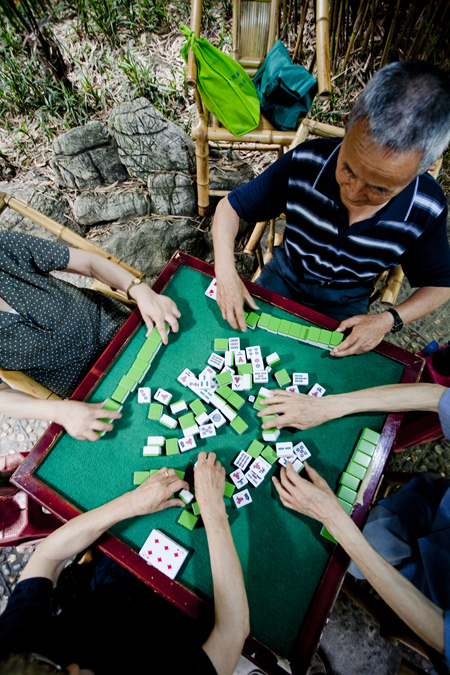
\includegraphics[scale=0.4]{pics/majiang2.png}     
        \end{center}
    \end{column}
    \end{columns}
\end{frame}

%% Appendices 
\appendix  % This resets the slide counters (appendixnumberbeamer)

    \begin{frame}<beamer:0>
        \frametitle{References}
        \def\newblock{}
        \bibliography{library.bib}
    \end{frame}

	\begin{frame}[label=threeLittlePigs]
	    \frametitle{Same wolf, different pigs}
	    \vspace{0.7}
	    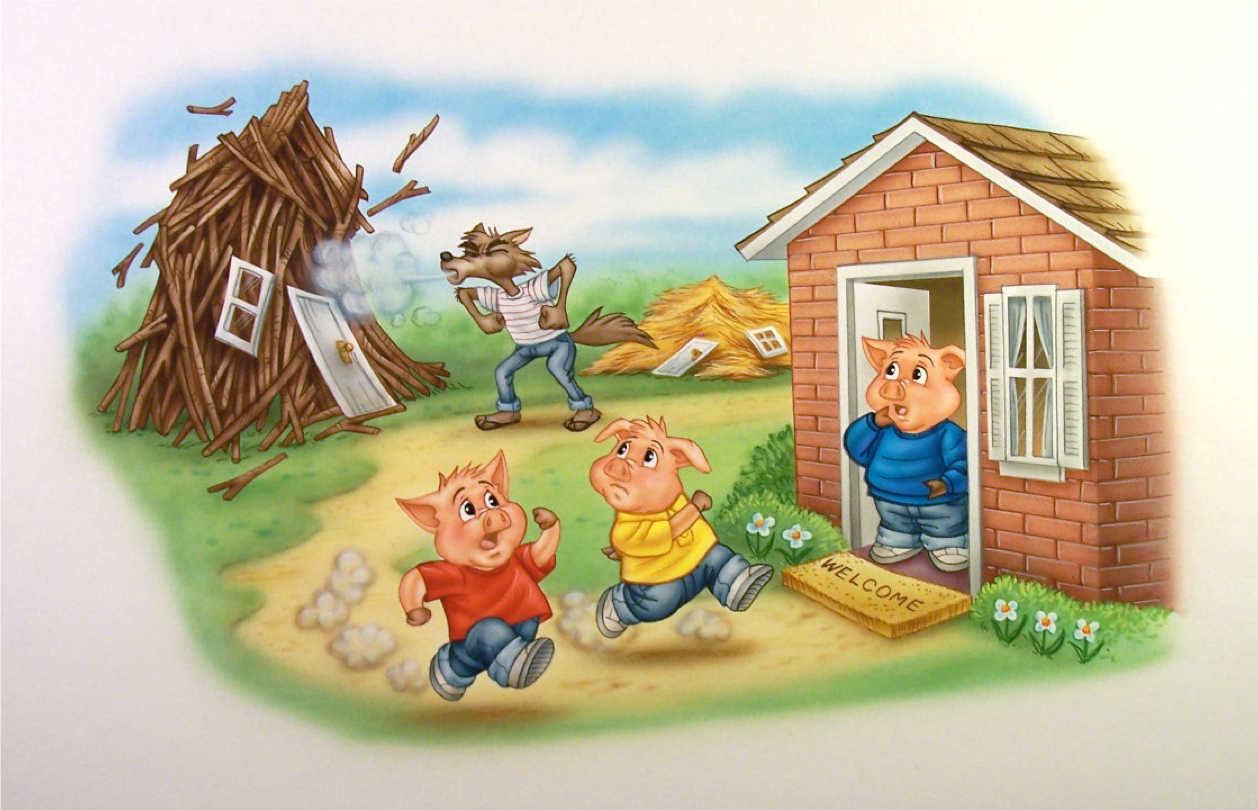
\includegraphics[scale=0.47]{pics/ThreeLittlePigs} \\		\hyperlink{simpleQuestion}{\beamergotobutton{Go back}}
	\end{frame}

    \begin{frame}[label=threeLittlePigs]
	    \frametitle{Same wolf, different pigs}
	    \vspace{0.7}
	    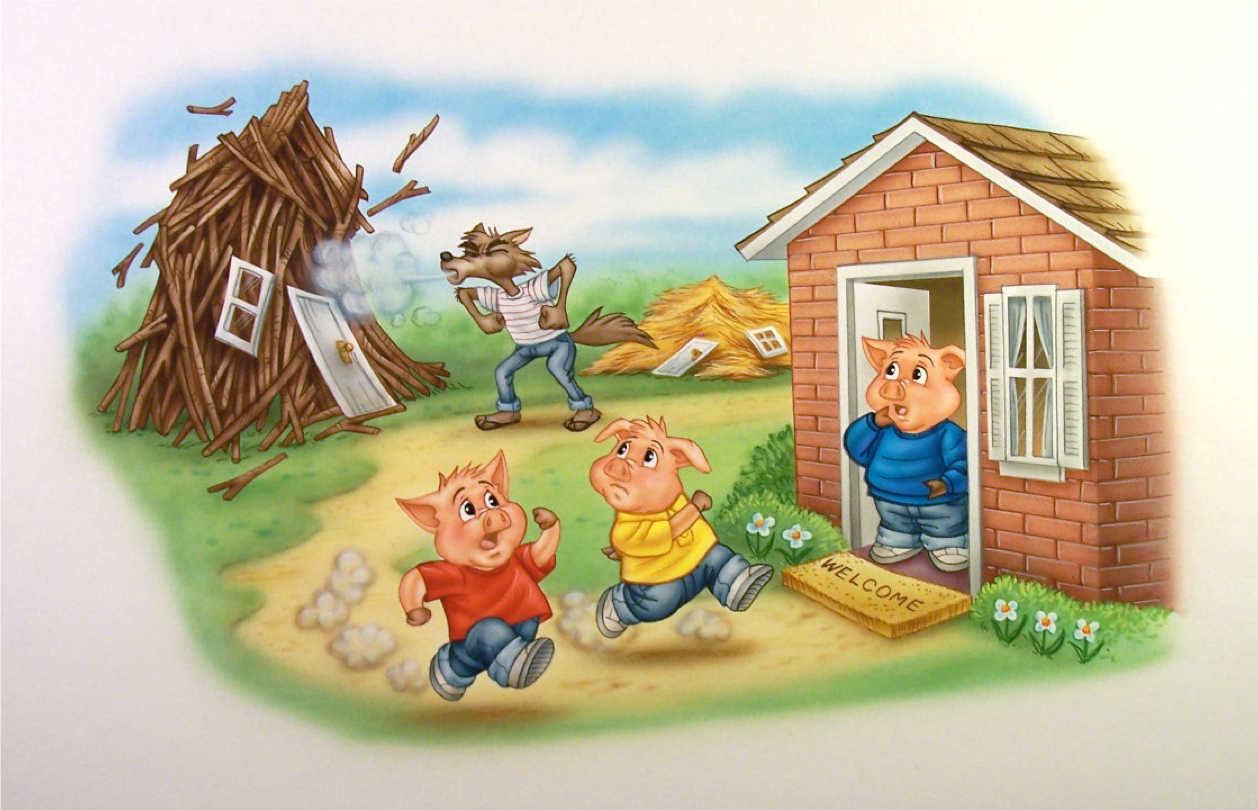
\includegraphics[scale=0.47]{pics/ThreeLittlePigs} \\		\hyperlink{simpleQuestion}{\beamergotobutton{Go back}}
	\end{frame}

\end{document}
